\chapter{Revisão da literatura}
%%%%%%%%%%%%%%%%%%%%%%%%%%%%%%%%%%%%%%%%%%%%%%%%%%%%%%%%%%%%%%%%%%%%%%%%%%%%%%%%%%%%%%%%%%%%%%%%%%%%%%
Para melhor didática e objetivando melhor compreensão dos temas abordados neste trabalho, a revisão bibliográfica foi dividida em cinco partes. A primeira etapa apresenta o sistema de perfuração de poços petrolíferos e seus componentes. Na segunda, é abordado o conceito de Desgaste erosivo e os atributos (variáveis) que propiciam sua ocorrência. A terceira parte discute sobre a técnica de simulação fluidodinâmica computacional. Na quarta parte são demonstrados os métodos de análise de risco para elaboração de cenários probabilísticos. Na quinta parte, é demonstrado o método de Planejamento estatístico por Superfície de resposta para obtenção de metamodelo de regressão. Por fim, são apresentados artigos científicos, dissertações e teses relacionados à estrutura da dissertação que servem como base para elaboração deste trabalho.

%%%%%%%%%%%%%%%%%%%%%%%%%%%%%%%%%%%%%%%%%%%%%%%%%%%%%%%%%%%%%%%%%%%%%%%%%%%%%%%%%%%%%%%%%%%%%%%%%%%%%%
\section{Perfuração de Poços Petrolíferos}

Na indústria de petróleo o processo para alcançar um reservatório subterrâneo de hidrocarbonetos através da construção de um poço é comumente referido como “perfuração”. A perfuração é uma das etapas de um projeto de exploração de um campo petrolífero, sendo geralmente a fase mais custosa. Um poço pode ter diferentes finalidades, tais como: estratigráfico, que visa fornecer informações sobre a estratigrafia e litologia das rochas; pioneiro, que tem como objetivo explorar áreas não mapeadas anteriormente; de injeção, utilizado para injetar fluidos no reservatório a fim de aumentar a produção; e o de produção, destinado a extrair e coletar hidrocarbonetos do reservatório (\cite{thomas}).

O processo de perfuração envolve diversos equipamentos e técnicas associadas. A sonda de perfuração possui sistemas acoplados e equipamentos com aplicações específicas que são os responsáveis pela perfuração. Para se perfurar uma formação rochosa é necessário o uso de brocas, que são equipamentos responsáveis por promover a ruptura e desagregação das rochas. A broca é situada na extremidade da coluna de perfuração e sofre um movimento de rotação, gerado pelo Motor de fundo ou por uma mesa rotativa e transmitida pela coluna. Essa energia, em forma de rotação e peso aplicados sobre a broca de forma contínua promove a ruptura e desagregação das rochas e, como resultado, gera pequenos fragmentos denominados “Cascalhos”, que são carreados do poço até a superfície pela circulação do Fluido de perfuração. Através da ação de uma bomba, o fluido de perfuração é injetado através da cabeça de injeção e percorre a coluna de perfuração passando pelos noodles da broca e, por fim, retorna para a superfície através do espaço anular formado pelas paredes do poço e a coluna (Figura \ref{fig:esquemaseparacao}) \cite{thomas}.


O fluido de perfuração percola por todo o poço, desempenhando diversas funções e retorna à superfície pela região anular carreando os fragmentos de rocha, para que na superfície passe por um processo de tratamento para separação sólido-líquido. A separação sólido-líquido tem por finalidade promover a máxima recuperação do fluido de perfuração para posterior reutilização, bem como a máxima limpeza dos cascalhos para posterior descarte. Ao carrear os cascalhos provenientes da perfuração, o fluido de perfuração deve passar por um processo de tratamento na plataforma para que possa retornar a operar no poço, por outro lado, o cascalho necessita de tratamento para que seja descartado sem danos ao meio ambiente. Conforme citado \citeonline{ROBINSON}), os principais componentes de um sistema de tratamento são as peneiras vibratórias, desgaseificador, desareiador, dessiltador, mudcleaner e centrífuga. Cada um desses equipamentos tem a função de remover sólidos com granulometrias específicas. É importante ressaltar que nem sempre todos esses componentes são utilizados, podendo variar de acordo com as necessidades do sistema de tratamento em questão.

\begin{figure}[H]
    \centering
    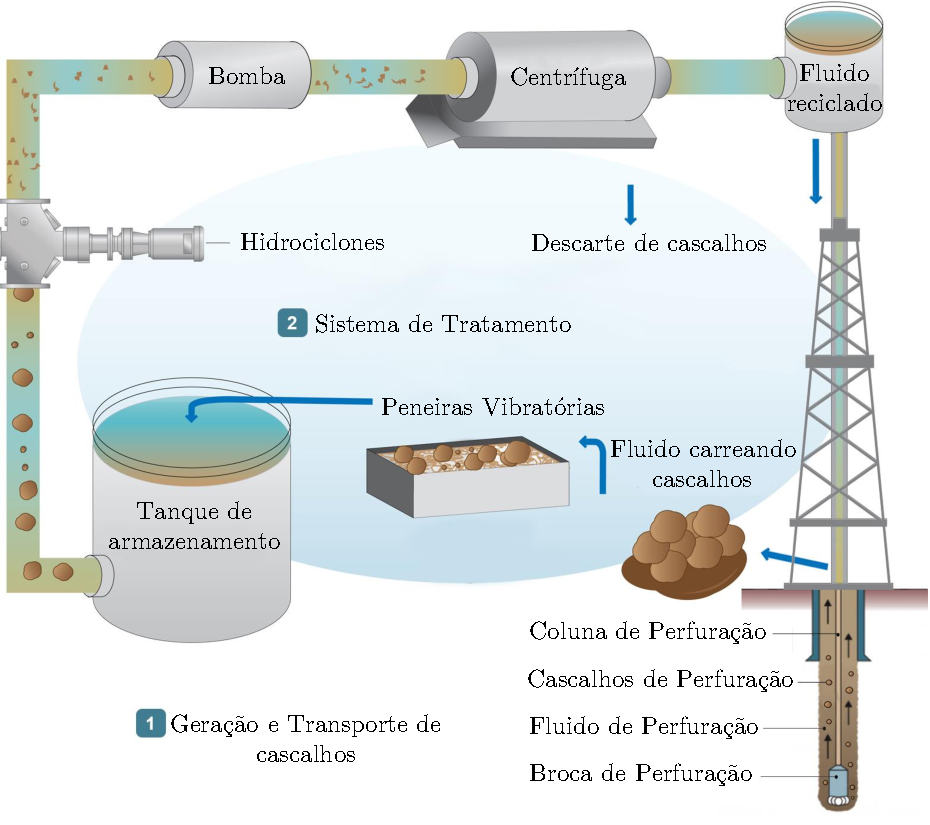
\includegraphics[scale=0.94]{Figuras/esquemaseparacao.pdf}
    \caption{Perfuração de Poços de Petróleo.}
    \legend {Fonte: Adaptado de \citeonline{rbn} e \citeonline{jwce}}
    \label{fig:esquemaseparacao}
\end{figure}

%%%%%%%%%%%%%%%%%%%%%%%%%%%%%%%%%%%%%%%%%%%%%%%%%%%%%%%%%%%%%%%%%%%%%%%%%%%%%%%%%%%%%%%%%%%%%%%%%%%%%%
\subsection{Fluido de Perfuração}

Os fluidos de perfuração são classificados de acordo com o constituinte que apresenta maior proporção em sua mistura, geralmente entre 60\% a 90\% de seu volume físico. Os fluidos são constituídos por uma fase continua que pode ser água, óleo ou gás, a essa fase são adicionados produtos químicos e materiais sólidos que auxiliam a alcançar propriedades específicas necessárias para aumentar a eficiência na operação de perfuração de poços \cite{thomas}.

Os fluidos de perfuração devem possuir características específicas de maneira a garantir uma perfuração eficiente e segura. Dentre as principais funções destacam-se: carrear os cascalhos de perfuração e permitir sua separação na superfície, resfriar a broca e a coluna de perfuração, reduzir o atrito entre a coluna de perfuração e as paredes do poço, manter a estabilidade do poço exercendo pressão hidrostática sobre as formações, para evitar influxo de fluidos da formação para o poço \cite{silva}. No trabalho de \citeonline{pereira}, foi analisada a vazão dos fluidos de perfuração em diferentes profundidades, conforme a Tabela \ref{tab:vazaofluido}.

\begin{table}[!h]
\caption{Vazão do fluido de Perfuração.}
\begin{tabular*}{\textwidth}{@{\extracolsep{\stretch{1}}}*{6}{c}@{}}
   
  \toprule
  Sonda & Fase  & Profundidade do Poço & Vazão do fluido de Perfuração \\
  \midrule
  número&número  & metros &	m³/h \\
  1  &	2 	&2272 &	91\\
 2&	3 	&1619&	98\\
3 &	2 &	610&	82\\
4 &	2&	1282&	91		\\

  \bottomrule   
\end{tabular*}
\label{tab:vazaofluido}
\legend {Fonte: Adaptado de \citeonline{pereira}}
\end{table*}
\end{table}

O fluido de perfuração é a primeira barreira de segurança do poço no processo de perfuração. A densidade do fluido é o parâmetro que regula a pressão hidrostática no poço. Dependo do método de perfuração adotado, a pressão hidrostática gerada pela coluna de fluido no poço, deve ser superior a pressão de poros da formação, afim de evitar influxos, e inferior a pressão de fraturamento da rocha, com o objetivo de evitar a geração de falhamentos. Para que se alcance este valor de equilíbrio existe um estudo geológico prévio que determina a pressão de poros da formação e a pressão de fratura da mesma. A Tabela \ref{tab:densidadefluido}, apresenta as principais características físico-químicas dos fluidos de perfuração utilizados nas atividades de perfuração do Campo de Mexilhão, na Bacia de Santos.

\begin{table}[!h]
\caption{Características físico-químicas dos fluidos de perfuração (Campo de Mexilhão)}
\begin{tabular*}{\textwidth}{@{\extracolsep{\stretch{1}}}*{6}{c}@{}}
   
  \toprule
  & Peso do fluido  & Salinidade & Acidez ou basicidade  \\
   & g/cm³ & mg/L &	pH \\
  \midrule
  Fluido de perfuração SCOL  &	1,44 	&87.000 &	10,0&\\
 Fluido de perfuração catiônico&	1,38 	&103.380&	11,5\\
Fluido de perfuração convencional &	1,07 &	5.000&	9,0\\
Fluido de perfuração STA &	1,32&	85.000&	9,5		\\
BR-MUL HT 1 &	1,50&	310.552&	-	\\
BR-MUL HT 2 &	1,45 &	94.645&	-	\\
  \bottomrule   
\end{tabular*}
\label{tab:densidadefluido}
\legend {Fonte: \citeonline{petrobras}}
\end{table*}
\end{table}


A Reologia desempenha um papel fundamental para otimização e eficiência dos fluidos de perfuração. A Reologia pode ser definida como a ciência que estuda a deformação e o fluxo da matéria. Muitas expressões matemáticas estão propostas na literatura para modelagem  do comportamento reológico de fluidos não newtonianos \cite{reology}.  

Os modelos reológicos descrevem o comportamento da viscosidade do fluido em relação a uma tensão aplicada. Geralmente o modelo de  Bingham e Herschel-Bulkley
representam as características de fluxo de um fluido de perfuração (Figura \ref {fig:bingham}). No modelo de Bingham, é necessário que se alcance a tensão crítica, isto é, tensão mínima para que o fluido comece a
escoar ou entre em movimento. Isto pois, quando o fluido se encontra em repouso, sem sofrer nenhum estado de tensões, a viscosidade aumenta consideravelmente. Ao se aplicar uma tensão mínima de cisalhamento o fluido passa a ter uma viscosidade menor, isto é, a tensão aplicada ao fluido passa a ser proporcional a deformação do mesmo (Fluido newtoniano), mantendo a viscosidade constante a partir desta tensão de cisalhamento mínima. O modelo de Herschel-Bulkley
também necessita de uma tensão de cisalhamento mínima para escoar, porém inicialmente a tensão não é proporcional à deformação do fluido \cite{thomas}. 


\begin{figure}[H]
    \centering
    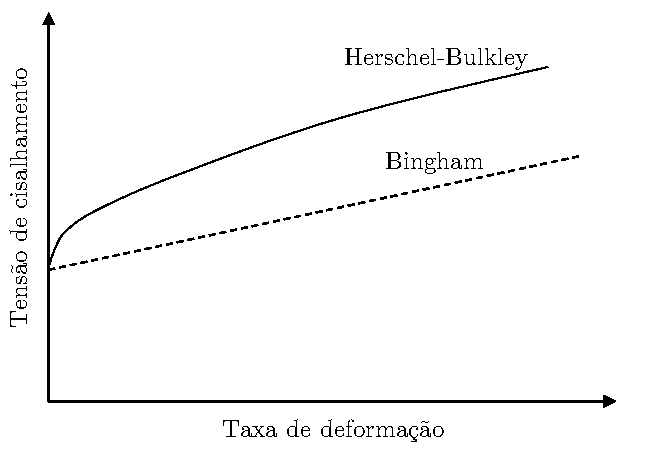
\includegraphics[scale=0.86]{Figuras/bingham.pdf}
    \caption{Modelos reológicos de Bingham e Herschel-Bulkley.}
    \label{fig:bingham}
    \legend{Fonte: Adaptado de \citeonline{reology}}
\end{figure}

A força gel é um parâmetro de natureza reológica que indica o grau de gelificação devido à interação elétrica entre partículas dispersas. A força gel inicial mede a resistência inicial para colocar o fluido em fluxo, ao passo que, a força gel final mede a resistência do fluido para reiniciar o fluxo a partir de um certo tempo em repouso. A diferença entre elas indica o grau de tixotropia do fluido. Os fluidos de perfuração apresentam esta característica tixotrópica, principalmente para manterem os cascalhos suspensos em casos de parada de fluxo, de modo a evitar desmoronamentos no poço \cite{pereira}. 

\citeonline{DYOVANI} comparou a variação na viscosidade aparente de diferentes fluidos de perfuração à base de Goma Xantana. Com base nas curvas de viscosidade foi possível descrever o
comportamento não Newtoniano e pseudoplástico dos fluidos de perfuração. Assim, devido a significante presença da
tensão limite de escoamento, os modelos que
melhor descreveram o comportamento dos fluidos
estudados foram os modelos de Herschel-Bulkley
e Bingham (Figura \ref{fig:fluidoperfura}).

\begin{figure}[H]
    \centering
    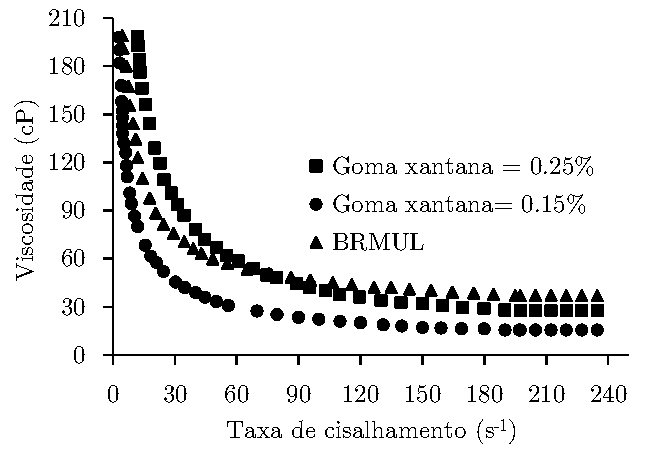
\includegraphics{Figuras/fluidoperfura.pdf}
    \caption{Comportamento reológico de três fluidos de perfuração de poços.}
    \label{fig:fluidoperfura}
    \legend{Fonte: adaptado de \citeonline{DYOVANI}}
\end{figure}

A Figura \ref{fig:fluidoperfura} demonstra que o comportamento da curva de
viscosidade aparente em função da taxa de
cisalhamento, para diferentes concentrações de Goma Xantana, é exponencial (caso fosse constante o fluido seria newtoniano).
Também é constatado o aumento da viscosidade aparente em maiores
concentrações de goma xantana. Em taxas de cisalhamento elevadas existe uma tendência a valores constantes de viscosidade. A
viscosidade aparente do fluido decresceu com o
aumento da taxa de deformação, por outro lado, em baixas taxas de deformação,
o fluido comporta-se semelhante a um corpo sólido, com viscosidade
tendendo a valores extremamente altos, os quais
decaem drasticamente com o aumento da taxa de cisalhamento.


%%%%%%%%%%%%%%%%%%%%%%%%%%%%%%%%%%%%%%%%%%%%%%%%%%%%%%%%%%%%%%%%%%%%%%%%%%%%%%%%%%%%%%%%%%%%%%%%%%%%%%
\subsection{Cascalhos de Perfuração}

Um dos principais resíduos da atividade de perfuração de poços de petróleo são os cascalhos de perfuração. A palavra cascalho de perfuração é uma tradução do inglês “rock cutting”. São fragmentos da formação originados pela ação da broca durante o processo de perfuração de poços e que são carreados para a superfície pelo fluido de perfuração. 
Os cascalhos de perfuração são gerados em todas as fases de perfuração de um poço. Para se estimar a geração de cascalhos de um poço diversas variáveis são levadas em conta. O volume oriundo da perfuração de um poço será dependente da profundidade, características geológicas, tipo de fluido utilizado e diâmetro do poço. Em suma, o volume total de cascalhos deve ser equivalente ao volume nominal do poço (volume do cilindro), ou seja, o volume de cascalho gerados é igual ao volume de poço perfurado por hora \cite{pereira}.

De acordo com \citeonline{fialho}, a partir de dados de perfurações terrestres, no Estado do Espírito Santo são gerados em média 0,13m³ de cascalhos por metro perfurado. \citeonline{schaffel}, determinou que os poços da bacia de campos apresentam aproximadamente entre 0,19m³ e 0,25 m³ de volume de cascalhos produzidos por perfuração. A Tabela \ref{tab:geracaocascalho}, demonstra o volume de cascalhos gerados no Poço P21 (Campo de Mexilhão).

\begin{table}[h]
\caption{Geração de cascalho do Poço P21 (Campo de Mexilhão)}
\begin{tabular*}{\textwidth}{@{\extracolsep{\stretch{1}}}*{6}{c}@{}}
 
  \toprule
    Fase& Profundidade & Diâmetro da broca & Diâmetro do furo & Cascalho Gerado\\
   & metros & polegada &polegada&m³\\
  \midrule
1&410&36”&30”&55\\
2&650&26”&20&82\\
3&2.000&17 ½”&13,375”& 266\\
4&4100&12 ¼” & 9,625”&180\\
5&4721&8 ½”&6,625”& 26\\

  \bottomrule   
\end{tabular*}
\label{tab:geracaocascalho}
\legend {Fonte: \citeonline{petrobras}}
\end{table*}
\end{table}

Os cascalhos de perfuração são resíduos granulares que apresentam características variáveis que vão depender de diversos fatores envolvidos durante a perfuração e, consequentemente, refletidos em suas propriedades físico-químicas. Segundo \citeonline{pereira} dentre os fatores que influenciam as características do cascalho, pode-se destacar: velocidade de perfuração, tipo de broca, diâmetro do poço, tipo de formação perfurada e peso do fluido. A depender desses parâmetros os cascalhos apresentam variabilidade nas características granulométricas (tamanho, forma) e parâmetros químicos, como a densidade. 
A composição química do cascalho é muito variada devido à heterogeneidade das formações atravessadas pela broca, assim como pela presença de contaminantes. Em um estudo com amostras de cascalhos de perfuração em um poço do Espirito Santo, \citeonline{fialho} obteve valores de massa específica equivalente a 2,58 g/cm³ (na fase de perfuração 1) e 2,67 g/cm³ (na fase de perfuração 3). \citeonline{pereira} encontrou valores próximos, com variação de 2,5 g/cm³ até 2,8g/cm³, tendo um valor médio de massa específica de 2,6 g/cm³. A Tabela \ref{tab:composicaocascalho} revela a proporção mineralógica dos cascalhos registrados em poços de perfuração por diversos autores. 


\begin{table}[!h]
\caption{Composição dos cascalhos de Perfuração.}
\begin{tabular*}{\textwidth}{@{\extracolsep{\stretch{1}}}*{6}{c}@{}}
 \toprule
   &ABBE et al (2009)& Medeiros (2010) & Leonard e Stegeman (2010)\\
  \midrule
SiO2&37,60&36,5&60,40 \\
Al2O3&13,54&11,5&10,40\\
Fe2O3&6,34&4,5&4,90\\
BaO&11,39&-&- \\
CaO&2,78&35,3&2,50\\

  \bottomrule   
\end{tabular*}
\label{tab:composicaocascalho}
\legend {Fonte: \citeonline{fialho}}
\end{table*}
\end{table}

Em geral, os cascalhos apresentam características físicas variadas a depender dos fatores citados anteriormente. Esses parâmetros físicos descrevem o tamanho do particulado, bem como fatores de forma da partícula (Esfericidade e razão de aspecto). A determinação da distribuição de tamanho e da forma de amostras de cascalhos de perfuração em diferentes profundidades (Grupo), realizadas por meio da técnica de análise dinâmica de imagens está apresentada na Tabela \ref{tab:granulometriacascalho}.


\begin{table}[!h]
\caption{Tamanho e forma (esfericidade) de amostras de cascalhos de Perfuração.}
\begin{tabular*}{\textwidth}{@{\extracolsep{\stretch{1}}}*{6}{c}@{}}
 \toprule
   Grupo &D[10]& D[50]& D[90]& D[médio]& Esfericidade \\
  \midrule
A - 2.376 &286,6 & 531,8 &1010,6& 588,2 & 0,787\\
B - 5.142 &345,5 &763,4 &1430,5 &828,6 & 0,765\\
C - 2.433 &169,3 &325,0 &682,4 &375,5  &0,783 \\
D - 2.529 &268,3 &468,3 &913,4 &753,4  &0,758 \\
E - 2.700 &273,8 &512,7 &1091,8 &599,1 & 0,792 \\
F - 3.201 &311,2 &562,7 &1257,0 &678,5  &0,777 \\
G - 3.312 &353,8 &661,8 &1342,3 &759,0 & 0,778 \\
H - 3.543 &315,5 &665,0 &1171,2 &713,2 & 0,776 \\
I - 3.564 &167,0 &321,1 &597,2 &352,4  &0,789 \\
J - 4.758 &339,7 &698,8 &1434,5 &805,5  &0,745 \\
K - 4.920 &335,1 &654,4 &1292,7 &732,9  &0,765 \\
L - 5.400 &521,3 &1107,47& 2105,5 &1222,5&  0,785\\
M - 4.824 &392,1 &719,1& 1554,0 &865,0 & 0,750 \\
N - 4.842 &356,0 &642,8& 1362,7 &757,6&  0,755\\

  \bottomrule   
\end{tabular*}
\label{tab:granulometriacascalho}
\subcaption{D[X]= diâmetro/ área abaixo do qual estão X\% das partículas (\mu  m).

D[médio] = diâmetro / X área médio (\mu  m).

Esfericidade (SPHT) = relação entre a área da partícula e seu perímetro.}
\legend {Fonte: \citeonline{bortotti}}
\end{table*}
\end{table}

No estudo de \citeonline{bortotti}, o tamanho dos cascalhos variou de d[10] 169,3 µm
(areia fina) até [d90] 2105,5 µm (cascalho muito fino), tendo diâmetro médio de
700,9 µm (areia grossa). Em relação ao fator de forma dos cascalhos,  75\%  das amostras apresentaram
esfericidade acima de 0,745. O grupo J foi o menos esférico,
tendo a esfericidade (SHPT) variando aproximadamente entre 0,511 D[10], 0,745 D[médio] e 0,888 D[90].
%%%%%%%%%%%%%%%%%%%%%%%%%%%%%%%%%%%%%%%%%%%%%%%%%%%%%%%%%%%%%%%%%%%%%%%%%%%%%%%%%%%%%%%%%%%%%%%%%%%%%%

\section{Erosão por partículas sólidas}
\label{cap:Erosão por partículas sólidas}


Erosão é a perda de material que constitui um equipamento ou tubulação de forma progressiva causada pelo impacto repetitivo de partículas sólidas ou liquidas contra a superfície de um corpo sólido. Isto ocorre devido ao arraste destas partículas por algum fluido até a superfície sólida do material alvo \cite{hutchings}.

No desgaste erosivo por partículas sólidas, várias forças de diferentes origens podem atuar sobre uma partícula em contato com uma superfície sólida (Figura \ref{fig:erosaoforca}). Partículas adjacentes podem exercer forças de contato e sob algumas condições, a gravidade pode exercer alguma influência. No entanto, a força dominante sobre uma partícula erosiva, que é a principal responsável por desacelerá-la da sua velocidade de impacto inicial, é a força de contato exercida pela superfície do material no momento de choque.

%%%%%%%%%%%%%%%%%%%%%%%%%%%%%FIGURA%%%%%%%%%%%%%%%%%%%%%%%%%%%%%%%%%%%%%%%%%%%%%%%%%%%%%%%%%%%%%%%
\begin{figure}[!h]
    \centering
    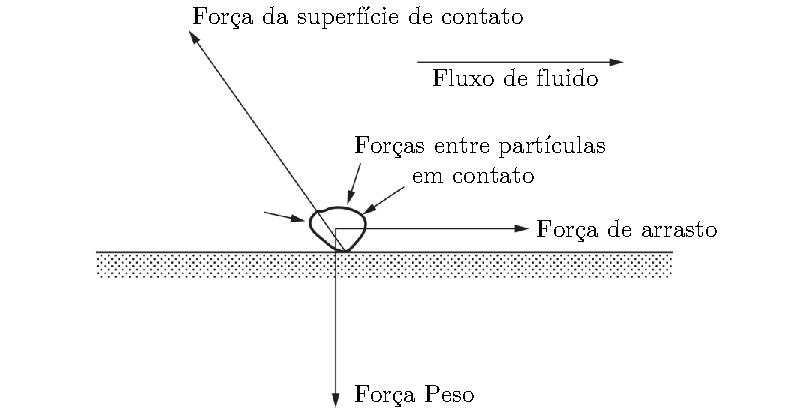
\includegraphics{Figuras/erosaoforca.pdf}
    \caption{Diagrama com as
forças sobre
partícula em contato com uma superfície sólida
}
\label{fig:erosaoforca}
\legend {Fonte: Adaptado de \citeonline{hutchings}}
\end{figure}
%%%%%%%%%%%%%%%%%%%%%%%%%%%%%FIGURA%%%%%%%%%%%%%%%%%%%%%%%%%%%%%%%%%%%%%%%%%%%%%%%%%%%%%%%%%%%%%%%

A erosão causada por partículas sólidas é um dos principais mecanismos de desgaste responsáveis por falhas em equipamentos presentes na indústria petrolífera. A produção de cascalhos durante a perfuração de poços pode causar danos erosivos consideráveis em tubulações, conexões, máquinas e equipamentos de separação sólido-líquido conectados a essas tubulações (Figura \ref{fig:erosaoperf}). O dano é pronunciado em regiões onde há uma mudança abrupta na direção do fluxo como curvas, válvulas e cotovelos que são partes integrantes da tubulação dos sistemas hidráulicos \cite {kumar}. 

\begin{figure}[H]
    \centering
    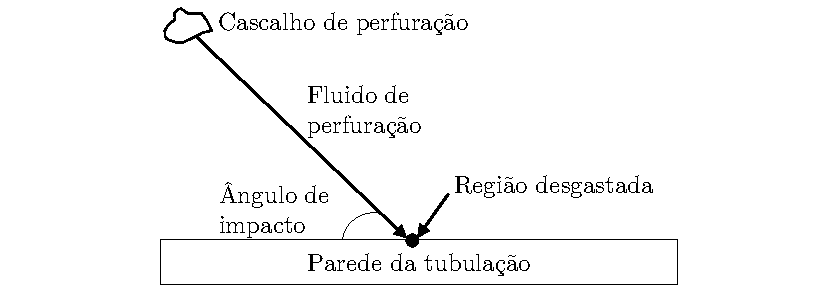
\includegraphics{Figuras/desgasteerosivoPerf.pdf}
    \caption{Desgate erosivo em linhas hidráulicas de perfuração de poços petrolíferos.}
\label{fig:erosaoperf}
\legend {Fonte: Adaptado de \citeonline{ANUR}.}
\end{figure}

O fenômeno da erosão é altamente complexo e uma ampla gama de parâmetros podem afetar a taxa de desgaste erosivo num determinado material. Vários pesquisadores mediram e quantificaram o efeito de diferentes parâmetros na erosão por partículas sólidas a qual pode ser classificada em quatro grupos de variáveis: as características da partícula erosiva, as características de impacto, as características de fluido e escoamento e as propriedades do material alvo. Estes grupos são apresentados em um diagrama típico de causa e efeito (Figura \ref{fig:erosaopeixe}) e são discutidos nos próximos parágrafos.

%%%%%%%%%%%%%%%%%%%%%%%%%%%%%FIGURA%%%%%%%%%%%%%%%%%%%%%%%%%%%%%%%%%%%%%%%%%%%%%%%%%%%%%%%%%%%%%%%%
\begin{figure}[H]
    \centering
    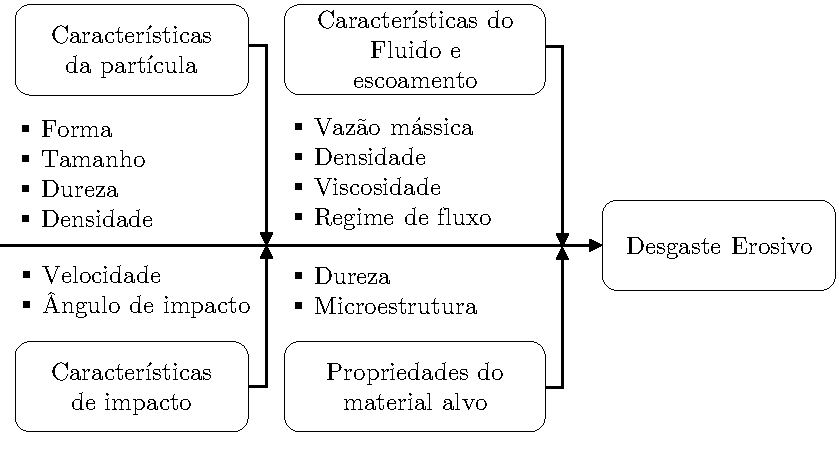
\includegraphics{Figuras/erosaopexie.pdf}
    \caption{Atributos que influenciam no desgaste erosivo.}
    \legend {Fonte: Adaptado de \citeonline{ANUR}.}
    \label{fig:erosaopeixe}
\end{figure}

%%%%%%%%%%%%%%%%%%%%%%%%%%%%%FIGURA%%%%%%%%%%%%%%%%%%%%%%%%%%%%%%%%%%%%%%%%%%%%%%%%%%%%%%%%%%%%%%%

A influência das propriedades e características das partículas foram estudadas em diversos trabalhos na literatura e são propriedades relevantes no desgaste erosivo. Em geral, partículas maiores resultam no aumento da taxa de erosão. Além da maior energia de impacto, o tamanho da superfície de contato tende a ser mais abrangente, levando a um maior desgaste no material \cite{zum} \cite{lieb}. Por outro lado, a alteração no tamanho das partículas pode influenciar nas direções de fluxo, o que resulta na mudança das regiões de colisão no material \cite {clark}. 

O estudo de \citeonline{hutchings} determinou que para calcular a taxa de erosão foi preciso verificar a forma das partículas erodentes, para isto propôs uma metodologia para a medição da forma das partículas utilizando um parâmetro (F), denominado fator de esfericidade. Este cálculo consiste na relação entre a área de projeção bidimensional das partículas e a área de um círculo com perímetro igual ao da projeção. No mesmo estudo, realizou experimentos envolvendo partículas esféricas e angulares. O impacto causado por partículas esféricas resultam em menor deformação localizada, ou seja, a taxa de erosão foi maior nos ensaios em que as partículas eram circulares \cite{walker}. 

Uma variável determinante na taxa erosiva é relação entre a dureza da partícula e a dureza do material alvo \cite{hutchings}. Em geral, partículas com menor dureza que o material causam menor desgaste comparado a partículas mais duras. \citeonline{divakar} alteraram a dureza do aço AISI 316 por laminação a frio e mostrou que um aumento na dureza diminui a erosão total em um testador de erosão a jato. Geralmente, com um aumento na dureza da partícula erodente, há um acréscimo na erosão total até certo limite, acima deste limite o aumento da dureza da partícula tem pouco efeito. \citeonline{levy} realizou testes de erosão em aço carbono AISI 1020 com dureza de 150 kgf/mm² utilizando partículas com diferentes níveis de dureza, ou seja, calcita, apatita, areia, alumina e carboneto de silício, no qual mostrou que acima de uma dureza de partícula de 700 kgf/mm², a taxa de erosão permaneceu constante. 

Em um fluxo multifásico líquido-sólido, a velocidade de impacto de uma partícula é uma função da velocidade de fluxo do fluido e a inércia da partícula em resistir à força de arrasto exercida pelo líquido. Deste modo, uma partícula de alta densidade apresenta uma velocidade de impacto maior do que uma de baixa densidade. Da mesma forma, a eficiência de colisão para partículas de alta densidade é maior do que as de baixa densidade em condições de teste idênticas. Portando, o efeito da colisão em maiores velocidades é o aumento da energia cinética de impacto, que juntamente com maior eficiência de colisão, resulta em maiores taxas de desgaste erosivo para partículas mais densas \cite {clark2}.
Uma das variáveis envolvidas no impacto é a velocidade da partícula no momento da colisão com o material erodido. Diversos pesquisadores constataram experimentalmente que a velocidade da partícula no momento do impacto com o material influencia diretamente na taxa de erosão. Isto está relacionado ao efeito da energia cinética das partículas erosivas \cite {lind}, \cite {trus}, \cite {finnie2}. No entanto, a partícula erodente tem que atingir uma velocidade crítica para induzir a deformação plástica na superfície do material alvo. Em velocidades de fluxo mais baixas, a maioria das partículas têm velocidades abaixo de um valor limite que resultam em deformação elástica, deste modo, é observado menor desgaste erosivo. Por outro lado, quando as partículas abrasivas atingem velocidade superior ao valor crítico, o impacto contínuo das partículas desenvolve plaquetas plasticamente deformadas que são removidas após impactos adicionais, o que significa maior desgaste erosivo \cite {yabuki}.

O ângulo de impacto, que é o ângulo entre a trajetória da partícula e a superfície do alvo, também pode afetar o desgaste erosivo no material. A variação da taxa de erosão em diferentes ângulos de impacto depende da ductilidade do material alvo. Em materiais dúcteis, a erosão máxima ocorre em ângulos de impacto entre 40° e 50°, enquanto para materiais frágeis a taxa de erosão máxima ocorre próximo de 90° \cite{albu}.

Diversos estudos, revelaram que quanto maior a concentração de partículas presentes no fluxo, maior a taxa de erosão devido ao número crescente de partículas que atingem a superfície da parede do alvo \cite{gandhi}. Ou seja, a taxa de erosão aumenta linearmente com a carga de partículas sólidas. Porém, existem situações em que o aumento da concentração de partículas erosivas pode gerar o aumento da quantidade de choques entre as partículas e a consequente diminuição de energia cinética de impacto, neste caso não ocorre a linearidade entre a concentração de partículas e o aumento de desgaste erosivo.  Outro caso é o fenômeno de incubação, em que ocorre a deposição de partículas na superfície do material erodido em função do aumento de partículas no escoamento e das condições de viscosidade do fluido \cite{tsai}. 

A viscosidade do fluido possui influência direta nas trajetórias das partículas, nas velocidades de impacto e nos ângulos de impacto, sendo um fator que determina a eficiência de colisão erosiva, isto é, a relação entre a quantidade total de partículas e a quantidade de partículas que efetivamente impactam contra a superfície do material alvo. Fluidos viscosos aumentam a flutuabilidade das partículas sólidas mantendo-as suspensas durante o fluxo. No caso de fluxos com líquidos menos viscosos, as partículas sólidas tendem a se depositar na superfície do material erodido \cite {yabuki}. Ou seja, significa que geralmente a perda de material é reduzida com a diminuição da viscosidade do fluido. No entanto, o efeito de viscosidade depende da velocidade do líquido. Em baixas velocidades superficiais (18, 27, 35 m/s), a perda de metal aumentou com o aumento da viscosidade do líquido, enquanto diminuiu em altas velocidade (45 m/s) \cite {yabuki}. \citeonline{kowsari} propuseram que, em uma velocidade muito alta (110 m/s), um aumento na viscosidade causa uma diminuição na erosão devido a dois efeitos viscosos. Primeiro, o aumento da viscosidade altera a zona de estagnação e, assim, reduz a energia de impacto das partículas e a capacidade erosiva. Em segundo lugar, uma maior viscosidade de fluido aumenta número de equilíbrio de momento, conforme, causando uma maior tendência das partículas seguirem as linhas de corrente. Isso, por sua vez, diminue o ângulo de impacto local na parte inferior do canal e reduz a taxa de erosão.

O impacto das partículas contra o material erodido é mais frequente em condições de fluxo turbulento. Assim, em fluxos laminares a taxa de desgaste é relativamente reduzida, pois neste regime de escoamento as partículas se movem paralelamente à superfície do material, diminuindo a possibilidade de geração de condições em que ocorrem impactos diretos em sua superfície.

A microestrutura do aço desempenha um papel importante na taxa de erosão. Dados de taxa de erosão normalizados indicam que a perlita é mais eficaz na resistência à erosão do que a ferrita, devido à sua estrutura lamelar, que é capaz de absorver a energia das partículas impactantes \cite{yabuki}.



%%%%%%%%%%%%%%%%%%%%%%%%%%%%%%%%%%%%%%%%%%%%%%%%%%%%%%%%%%%%%%%%%%%%%%%%%%%%%%%%%%%%%%%%%%%%%%%%%%%%%%%%%%


\section{Simulação Fluidodinâmica computacional (CFD)}
\label{Simulação Fluidodinâmica computacional (CFD)}

Podemos geralmente definir fluidodinâmica computacional (CFD) como simulações feitas a partir de computador, através de resolução de equações, com objetivo de analisar sistemas complexos que incluem transferência de calor, fluxos de fluidos e reações químicas \cite{versteeg}. O modelo de simulação objetiva representar em um ambiente computacional as características que o sistema apresentaria em condições semelhantes de contorno. 


Os códigos para simulação fluidodinâmica computacional são voltados para algoritmos numéricos configurados em interface gráfica de usuário, que facilitam a inserção dos parâmetros de entrada, o processo de solução e a visualização dos resultados da simulação. As principais etapas de um pacote CFD são definidas como: identificação do problema, pré-processamento, solução e pós-processamento (Figura \ref{fig:etapascfd}). O métodos utilizado em CFD para resolução das equações é método dos volumes finitos (MVF), que se baseia na aplicação de integrais para cálculos de conservação de energia, massa e momentum, podendo prever numericamente o comportamento de fluxos multifásicos e turbulentos relativamente complexos.  As próximas seções apresentam um breve resumo das etapas envolvidas em uma simulação computacional CFD.

%%%%%%%%%%%%%%%%%%%%%%%%%%%%%FIGURA%%%%%%%%%%%%%%%%%%%%%%%%%%%%%%%%%%%%%%%%%%%%%%%%%%%%%%%%%%%%%%%
\begin{figure}[H]
    \centering
    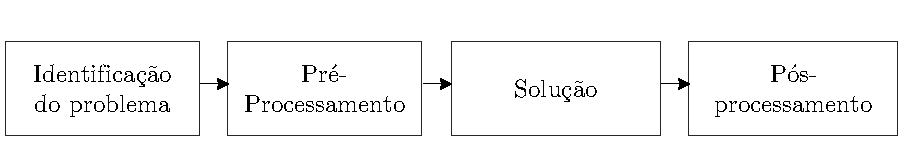
\includegraphics{Figuras/cfd.pdf}
    \caption{Etapas da simulação fluidodinâmica computacional.}
    \legend {Fonte: \citeonline{versteeg}}
    \label{fig:etapascfd}
\end{figure}
%%%%%%%%%%%%%%%%%%%%%%%%%%%%%FIGURA%%%%%%%%%%%%%%%%%%%%%%%%%%%%%%%%%%%%%%%%%%%%%%%%%%%%%%%%%%%%%%%%%

É necessário definir inicialmente qual o problema em questão que necessita ser modelado. Isso pode resultar em simplificações na criação da geometria, de forma a evitar gasto de tempo e capacidade computacional em regiões que não são de interesse no estudo fluidodinâmico. Na fase de pré-processamento é realizada a elaboração da geometria através de desenho assistido por computador (CAD). A geometria deve caracterizar toda a região onde ocorre o escoamento \cite{petrila}.

O método de volumes finitos é utilizado em simulações CFD, este consiste na divisão do espaço físico em blocos separados conhecido como malha computacional. Esta é a fase da discretização do modelo, onde a estrutura geométrica é dividida em volumes de controle, os quais representam a porção onde são empregados métodos numéricos na resolução das equações. Após definido os volumes de controle, são configurados os parâmetros físicos utilizados pelo solver para o cálculo do problema físico estudado \cite{anderson}.

A Solução é a etapa de processamento onde ocorre a resolução das equações no espaço e no tempo, ou seja, as equações de conservação de massa, energia e quantidade de movimento. Todas as grandezas físicas são calculadas em um mesmo passo do tempo (iteração), de forma que são feitas até atingir a convergência ou número de iterações estabelecidas \cite{batchelor}.

Na etapa de pós-processamento, os resultados são apresentados e analisados. Deste modo, é possível visualizar os valores e apresentar os resultados de interesse de forma iterativa, obtendo valores de grandezas físicas em qualquer parte do volume de controle do material estudado \cite{versteeg}.


\subsection{Modelagem Matemática e Computacional dos Escoamentos}

Na perfuração de poços de petróleo, ao fragmentarem e serem carregados pelo fluido de perfuração, os cascalhos juntamente com o fluido formam um sistema multifásico de escoamento. A modelagem computacional apresenta as equações governantes do problema, as condições de contorno, e as equações constitutivas necessárias que complementam a modelagem.

Quando o escoamento é laminar, é facilmente modelado e simulado pelo programa. Porém, as simulações de escoamentos turbulentos apresentam maior custo computacional e complexidade envolvida. O escoamento turbulento é caracterizado como uma condição irregular de escoamento, ou seja, são instáveis, com múltiplas escalas, rotacionais, tridimensionais, com alta difusibilidade e de forma contínua \cite{turb}.
Dado a importância da caracterização de escoamento turbulento, foram desenvolvidos métodos de solução computacional para representação desse fenômeno físico. O escoamento turbulento pode ser dimensionado por três diferentes técnicas: Simulação Numérica Direta (DNS) Simulações de Grandes Escalas (LES) ou através das equações de Navier-Stokes com médias de Reynolds (RANS) \cite{turb}.

A modelagem Navier-Stokes com médias de Reynolds (RANS) é a mais utilizadas para modelagem de escoamento turbulento. Este modelo de cálculo de turbulência resulta em menor esforço computacional comparado aos demais \cite{versteeg}. As equações são caracterizadas pela decomposição da velocidade em termos de um valor médio e de flutuação. O Tensor específico de Reynolds ocorre como resultado dos processos de média de Reynolds aplicados às equações de conservação de massa e de quantidade de movimento. Para determinação do tensor específico de Reynolds se faz necessário o uso de modelos de turbulência, dentre os modelos existentes destacam-se:  k-ω; k-ω SST; k-Є Standard; k-Є RNG; k-Є Realizable \cite{versteeg}. O modelo k-Є Standard usa duas equações de transporte,  é o modelo mais utilizado atualmente, pois possui um baixo custo de processamento computacional e descreve de forma satisfatória escoamentos turbulentos.

O escoamento multifásico é caracterizado pela presença de mais de uma fase num determinado sistema, portanto, na perfuração de poços de petróleo, ao fragmentarem e serem carreados pelo fluido de perfuração, os cascalhos juntamente com o fluido formam um sistema multifásico de escoamento. Assim, para um fluxo líquido-sólido, a fase contínua é dominante durante o escoamento. Já a fase dispersa é a fase carreada pelo contínuo. Deste modo, num fluxo envolvendo fluido de perfuração e cascalhos, o fluido é a fase contínua e os cascalhos a fase dispersa.  As técnicas de modelagem de fluxo multifásico são divididas em dois grupos: Euleriano-Euleriano e Euleriano-Lagrangeano.

No Modelo Euleriano-Euleriano, as fases envolvidas são tratadas matematicamente como fases continuas interpenetrantes \cite{ansys}. Neste modelo o local onde se encontra uma fase não pode ser ocupado pela outra fase. Já no modelo Euleriano-Langrageano (Modelo de fase discreta), uma das fases é tratada como continua (Euleriano), resolvendo as equações de Navier-Stokes. A outra fase é considerada discreta (Langrageana), cujas equações de movimento são baseadas na segunda Lei de Newton para o deslocamento de partículas. Este modelo é utilizado no presente trabalho e será descrito a seguir.

A forma de modelagem Euleriana-Lagrangeana no Ansys é denominada DPM (Discrete Phase Model) ou Modelagem da Fase Discreta. Para utilização deste modelo é necessário que a fase discreta tenha proporção volumétrica menor que 10\% em relação a fase contínua, de modo que as partículas no sistema não influenciem no fluxo da fase contínua. Assim, o equacionamento da trajetória da partícula lagrangeana é calculado separadamente da fase contínua. Para se prever a trajetória e direção de movimento das partículas (Velocidade e posição), faz-se a integral do balanço de forças na partícula em relação a sua inércia (com base na segunda lei de newton) de acordo com a equação \ref{eqn:euleriano} (unidades em SI), utilizando um referencial Langrageano. Essas integrais são resolvidas gradualmente ao longo de cada passo de tempo das simulações.

\begin{equation}
\frac{\partial uv}{\partial{}t}=Fd (v-uv)+ \frac{gx(\rho\rho -\rho )} {\rho\rho}+Fi
\end{equation}
\begin{equation}
FD=\frac{18u}{pp {dp}^2} \frac{CdRe}{24}
\label{eqn:euleriano}
\end{equation}

Onde:

 Fi= é um termo de aceleração adicional (força por massa de uma unidade de partícula;
 
 Fd (u-uv)= é a força de arrasto por massa de uma unidade de partícula;
 
 v= é a velocidade da fase contínua;
 
 uv= é a velocidade da partícula;
 
 u= viscosidade molar do fluido;
 
 p= é a densidade do fluido;
 
 pp= é a densidade da partícula;
 
 dp= é o diâmetro da partícula.


%%%%%%%%%%%%%%%%%%%%%%%%%%%%%%%%%%%%%%%%%%%%%%%%%%%%%%%%%%%%%%%%%%%%%%%%%%%%%%%%%%%%%%%%%%%%%%%%%%%%%%

\subsection{Simulação numérica para previsão do desgaste erosivo}

A previsão de erosão é sempre uma tarefa difícil na indústria de petróleo e gás devido ao desafio de entender, sob circunstâncias complexas de comportamento de fluxo, a distribuição das partículas sólidas ao longo do escoamento e os locais propensos ao impacto nos diversos equipamentos envolvidos nas etapas de exploração e produção. Outrossim, diversos parâmetros podem influenciar este tipo de desgaste em diferentes magnitudes, como demonstrado no Capítulo \ref{cap:Erosão por partículas sólidas}.

A complexidade da previsão de erosão aumenta significativamente em fluxos multifásicos em que gases, líquidos e sólidos podem estar presentes simultaneamente no escoamento.  Este regime de fluxo é dependente do tamanho da tubulação, ângulos de inclinação e propriedades do fluido que afetam significativamente as regiões e velocidade de impacto das partículas sólidas no material.

Nos últimos anos, a simulação fluidodinâmica computacional emergiu como uma ferramenta preferida para a previsão de erosão. Isto se deve ao fato de ser capaz de reproduzir condições de fluxos multifásicos e turbulentos e permitir o rastreamento da trajetória de partículas nestes sistemas \cite{yuhan} \cite {Parsi}. Deste modo, é possível obter uma compreensão dos efeitos do fenômeno físico erosivo através da identificação dos locais mais propenso ao impacto das partículas, prever a taxa máxima de erosão e o efeito de diferentes parâmetros no desgaste erosivo. A abordagem CFD também surge como uma alternativa de estudo em casos que a criação de uma análise experimental é difícil. A Figura \ref{fig:cfderosao}, demonstra uma simulação de fluxo de fluido ao longo de uma turbulação de geometria curva. Deste modo, é possível verificar que a simulação CFD determinou os locais de impacto das partículas sólidas no material e foi capaz de prever as regiões com maiores taxas de desgaste erosivo, representadas pelo gradiente de cores. Em contrapartida, para um estudo experimental as regiões de maiores desgastes são justamente os locais onde ocorre a falha do material.

%%%%%%%%%%%%%%%%%%%%%%%%%%%%%FIGURA%%%%%%%%%%%%%%%%%%%%%%%%%%%%%%%%%%%%%%%%%%%%%%%%%%%%%%%%%%%%%%%
\begin{figure}[H]
    \centering
    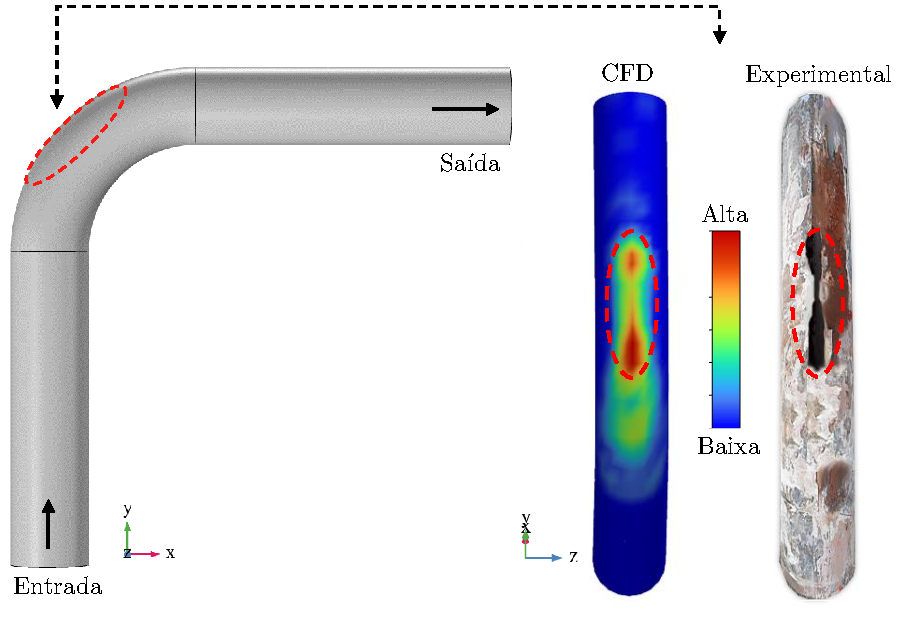
\includegraphics{Figuras/cfderosao.pdf}
    \caption{Simulação fluidodinâmica computacional para a previsão do desgaste erosivo.}
    \label{fig:cfderosao}
    \legend {Fonte: o autor.}
\end{figure}
%%%%%%%%%%%%%%%%%%%%%%%%%%%%%FIGURA%%%%%%%%%%%%%%%%%%%%%%%%%%%%%%%%%%%%%%%%%%%%%%%%%%%%%%%%%%%%%%%

Diversos estudos para o desenvolvimento de equações e modelos analíticos para avaliar a erosão em condições de escoamento monofásico e multifásico foram publicados \cite {oka} \cite {dnv} \cite {finnie} \cite{maclaury}. Porém cada modelo foi desenvolvido sob condições especificas de experimentos, o que influencia diretamente nas variáveis consideradas no cálculo erosivo, haja vista que existem muitos fatores que podem afetar a taxa de erosão. Portanto, existe pouco consenso na literatura sobre a melhor forma de prever quantitativamente a taxa erosiva. Deste modo, a depender do tipo de material avaliado e as condições de escoamento existentes, é possível definir um modelo de erosão específico que atende melhor a previsão do desgaste erosivo com base em validação com dados experimentais.

No estudo de \citeonline{liuuh}, foram feitas simulações CFD para previsão de erosão em curvas de aço carbono com raio de curvatura de 90°, em escoamento turbulento líquido-sólido. Após comparação com vários outros quatro modelos encontrados na literatura, resultados experimentais e validações publicadas, o modelo de \citeonline{oka} se provou o mais adequado para as condições de validação entre modelo numérico e experimental para erosão em curvas de 90° de raio curto e sob as condições de escoamento estudadas. As equações que representam o modelo de Oka, se encontram dispostas a seguir: 

\begin{equation}
    E(\alpha) = g(\alpha)E90
    \label{equationoka}
\end{equation}
\begin{equation}
E90=K(aHv)^{k1b}  \left ( \frac{v}{v'} \right )^{k2} \left ( \frac{d}{d'} \right )^{k3} 
\end{equation}
\begin{equation}
g(\alpha)= (sin   \alpha)^{_{n1}}(1+Hv(1-sin  \alpha))^{^{n2}}
\end{equation}
\begin{equation}
n1=s1(Hv)^{q1}
\end{equation}
\begin{equation}
n2=s2(Hv)^{^{q2}} 
\end{equation}
\begin{equation}
k2=2.3(Hv)^{0.038} 
\end{equation}

Onde: 

E ($\alpha$) = é a taxa de erosão em determinado ângulo.

E90= é a taxa de erosão em ângulo de 90 graus (taxa de erosão na direção normal); 

g ($\alpha$) = função do ângulo de impacto (graus);

k, k1 e k3= são constantes determinadas pelas propriedades das partículas;

k2= é uma função da dureza do material e de propriedades da partícula;

V= velocidade de impacto da partícula (m/s);

D= diâmetro da partícula ($\mu$m);

V'= velocidade de referência do experimento de Oka (m/s);

D'= diâmetro da partícula de referência do experimento de Oka ($\mu$m);

Hv= é o número de dureza de Vickers do material alvo (em GPa).


%%%%%%%%%%%%%%%%%%%%%%%%%%%%%%%%%%%%%%%%%%%%%%%%%%%%%%%%%%%%%%%%%%%%%%%%%%%%%%%%%%%%%%%%%%%%%%%%%%%%%%%%%%%%%%%%%%%
\section{Análise de risco}

O risco pode ser entendido como uma função de incertezas envolvidas em um projeto, que para a indústria de Óleo e Gás podem ser geológicas, econômicas e tecnológicas, cujas análises possam ser integradas. O entendimento de risco de um projeto contribui para a tomada de decisão durante o processo de perfuração de poços. Sob a perspectiva de falha dos componentes, a quantificação de risco representa a otimização na determinação da manutenção preventiva, troca dos equipamentos se seleção adequada de equipamentos.

A análise de risco de um projeto de Perfuração de poço petrolífero requer informações detalhadas a respeito das propriedades e características relativas as rochas e fluidos de perfuração, sendo necessário o entendimento dos parâmetros fluidodinâmicos e petrofísicos integrados, que podem ser caracterizados através da simulação numérica computacional \cite{loschiavo}. Embora seja amplo, o conceito de incerteza utilizado neste trabalho está relacionado à falta de conhecimento dos valores precisos dos atributos que influenciam no desgaste erosivo, ou seja, a incerteza dos atributos causa incerteza na previsão do desgaste erosivo de um projeto de perfuração de poços. Deste modo, a combinação das variáveis aleatórias que influenciam no desgaste erosivo, em diversos cenários, resultam na quantificação de risco para tomada de decisão.

A etapa preliminar da análise de risco consiste na seleção e caracterização dos atributos geológicos e físicos a serem utilizados na análise de incertezas. A incerteza do atributo deve ser expressa através de sua distribuição de probabilidade para o processo de análise de risco. Na prática, os dados disponíveis geralmente não são suficientes para o correto conhecimento das variáveis analisadas. Em muitos casos são obtidos apenas os valores mínimos, prováveis e máximos dos atributos, através de dados amostrais ou estimados por especialistas (Engenheiros, geólologos, geofísicos e petrofísicos) ou a partir do conhecimento que se tem de poços vizinhos. Os atributos também podem ser definidos pela divisão ou multiplicação do valor mais provável \cite{steagall}.

A quantidade de variáveis de entrada do modelo determina o esforço e tempo computacional para simulações de cenários probabilísticos. Portanto, uma etapa essencial para a análise de risco é o estudo de sensibilidade, que consiste na definição dos atributos críticos, ou seja, as variáveis que mais exercem impacto na resposta da simulação numérica (desgaste erosivo). Esse processo tem por finalidade a redução do número de variáveis utilizadas no estudo. Dado que, a aplicação de todos os atributos incertos pode ser inviável computacionalmente, pois o número de simulações cresce com a quantidade de variáveis, e de mesma forma desnecessária, pois algumas variáveis podem causar impactos mínimos na quantificação de risco \cite{santoss2}. A análise de sensibilidade é um método que consiste em variar os atributos em um nível inferior e superior e observar o impacto desta variação na Função-objetivo, o que permite estimar quais fatores apresentam maior influência na resposta. O planejamento de Plackett-Burman pode ser utilizado para a triagem dos fatores, ou seja, determinar o impacto das variáveis sobre a função-objetivo, uma vez que são capazes de obter informações sobre os efeitos  principais e as interações entre as variáveis simultaneamente \cite{plackett}. Deste modo, utilizando o planejamento estatístico para a realização do estudo de sensibilidade, pode-se determinar os fatores críticos para aplicação dos métodos de combinação dos atributos para análise de risco.


\subsection{Método da Àrvore de Derivação}

A análise de risco baseada na Metodologia da Árvore de Derivação tem como base a simulação numérica de vários cenários possíveis, através da combinação de atributos. Os atributos são discretizados em níveis de incerteza, aos quais estão associadas determinadas probabilidades de ocorrência de acordo com sua distribuição de probabilidade \cite{madeira}. A Figura \ref{fig:arvorederivacao} demonstra uma árvore de derivação constituída por 2 atributos, ambos com três níveis de ocorrência com probabilidade associada.

\begin{figure}[H]
    \centering
    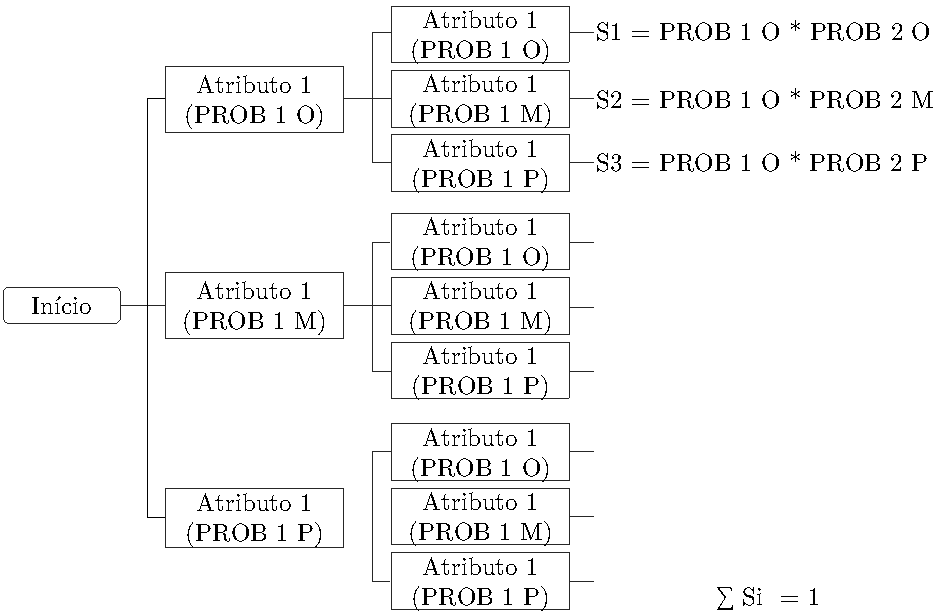
\includegraphics[scale=1]{Figuras/derivacao.pdf}
    \caption{Exemplo de árvore de derivação - 2 atributos com 3 níveis.}
    \legend {Fonte: Adaptado de \citeonline{madeira}}
    \label{fig:arvorederivacao}
\end{figure}

Todos os cenários representados na árvore são submetidos à simulação fluidodinâmica computacional.
A probabilidade de ocorrência de cada cenário de simulação fluidodinâmica corresponde ao produto das probabilidades de ocorrência dos níveis dos atributos presentes no modelo. Cabe citar que as probabilidades de ocorrência dos atributos são consideradas como independentes \cite{risso1}. 
O número total de modelos a serem simulados é definido pelo número de atributos e seus níveis de incerteza. De tal modo que, por exemplo, quatro atributos incertos com três níveis de incerteza resultam em $3^{4}$=81  modelos de simulação. A inclusão de um atributo aumenta o número de simulações exponencialmente, de acordo com a Figura \ref{fig:arvorederivacao2}.

\begin{figure}[!h]
    \centering
    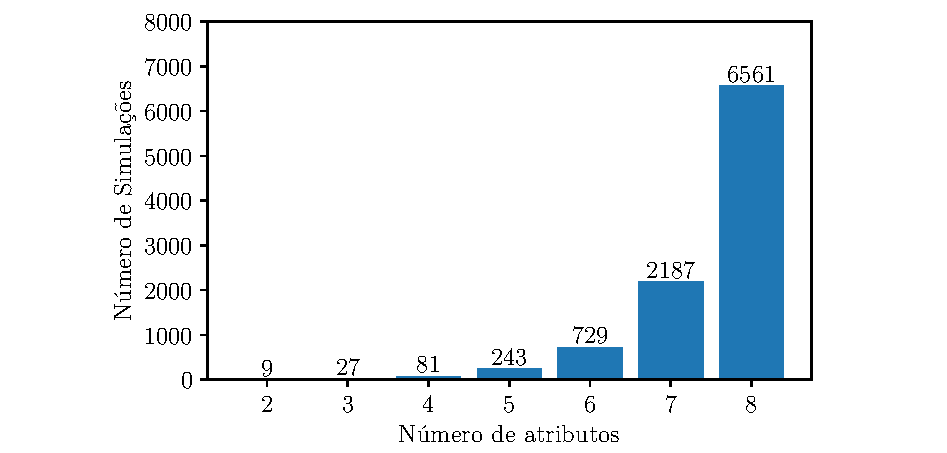
\includegraphics[scale=1]{Figuras/arvoredevr.pdf}
    \caption{Número de simulações para Àrvore de derivação com 3 níveis.}
    \legend {Fonte: Adaptado de \citeonline{madeira}}
    \label{fig:arvorederivacao2}
\end{figure}


A presença desnecessária de atributos pouco influentes incrementa o tempo computacional de processamento, devido ao aumento do número de modelos de simulação. Deste modo, os atributos que compõe a Àrvore de derivação são os definidos como críticos na análise de sensibilidade, ou seja, apenas os atributos que exercem influência significativa na Função-objetivo. Deste modo caso o número de atributos críticos seja elevado, a metodologia passa a ser custosa do ponto de vista computacional \cite{madeira}.

Após a realização das simulações e com base nos resultados, é possível realizar o tratamento estatístico necessário para obter a curva de risco de falha. Esse tratamento estatístico envolve a análise dos dados coletados durante a simulação, a determinação das probabilidades de falha em diferentes cenários e a construção da curva de risco, que representa a probabilidade de ocorrência da falha ao longo do tempo operacional. Essa curva de risco de falha é uma ferramenta valiosa para a tomada de decisões informadas e a implementação de medidas de mitigação de risco adequadas \cite{risso1}.


\subsection{Método de Monte Carlo}

O método de Monte Carlo é uma técnica estatística que envolve a amostragem aleatória de variáveis de entrada incertas. Essa abordagem é utilizada como uma ferramenta para gerar cenários diversos, nos quais são realizadas inferências estatísticas. Em outras palavras, a técnica de Monte Carlo é uma técnica para modelagem de cenários estocásticos (sujeito a alguma densidade de probabilidade). A amostragem aleatória é realizada nos atributos que exercem influência sobre o problema estudado e os valores são amostrados de acordo com sua distribuição de probabilidade de cada atributo (assumida ou estimada) \cite{hammers}.

Para o método de Monte Carlo, para cada cenário simulado, existe uma solução para o problema. Deste modo, os cenários realizados resultam em um espectro com a distribuição de probabilidades empírica das respostas. Para produzir uma estimativa consistente da função de distribuição de probabilidade para a resposta, é necessário simular um número elevado de cenários. Portanto, é imprescindível a obtenção de diversos valores aleatórios para os atributos de modo que os cenários realizados possam se adequar à distribuição dos atributos \cite{Srikanta}


As etapas do método de Monte Carlo são, basicamente:

\begin{itemize}
  \item Gerar sorteios e obter amostras de objetos estocásticos com uma determinada densidade de
probabilidade;
  \item Obter o resultado da Função-objetivo de cada cenário realizado pelos sorteios;
  \item Agregar os resultados para obter dados estatísticos para análise;
  \item Assegurar que os resultados são representativos, ou seja, evidenciar o número de sorteios ideal que reproduzam de maneira fiel a distribuição dos atributos e que as estatísticas da resposta permaneçam dentro de uma margem de erro aceitável.
\end{itemize}

A simulação numérica por fluidodinâmica computacional para previsão do desgaste erosivo dos cenários gerados pela técnica de Monte Carlo é inviável do ponto de vista computacional, devido ao elevado número de sorteios. Por esta razão, é necessário recorrer a metodologias que resultem nas respostas com menor esforço computacional e estatisticamente confiável em relação ao modelo de simulação numérico. Assim, os metamodelos (\textit{Proxy models} ou \textit{Surrogate models}) se apresentam como uma excelente alternativa à simulação de Monte Carlo como ferramenta subsidiária da metodologia. Os metamodelos são aplicados para substituirem modelos de simulação numérica e podem ser usados para diminuição do esforço e tempo computacional empregados para análise de risco. Na próxima seção são abordados os métodos de geração de metamodelos através da metodologia de Superfície de Resposta.
%%%%%%%%%%%%%%%%%%%%%%%%%%%%%%%%%%%%%%%%%%%%%%%%%%%%%%%%%%%%%%%%%%%%%%%%%%%%%%%%%%%%%%%%%%%%%%%%%%%%%%%%%%%%%%%%%%%

\section{Metamodelos}

As Simulações fluidodinâmicas para previsão de desgaste erosivo, necessitam de muito esforço computacional, principalmente nos processos de análise de risco que demandam diversos cenários probabilísticos.
Os metamodelos (\textit{Proxy models} ou \textit{Surrogate models}), portanto, se apresentam como ferramentas subsidiárias da análise de risco, com objetivo de reduzir o número de simulações requisitadas para elaboração e previsão dos cenários probabilísticos necessários para composição das curvas de risco de falha por desgaste erosivo.
Neste trabalho, o planejamento estatístico é aplicado em duas ocasiões. Inicialmente o seu emprego tem como finalidade realizar a triagem dos atributos incertos, determinando quais fatores apresentam maior influência na função-objetivo, com objetivo de reduzir o número de simulações necessárias nas etapas seguintes de análise \cite{Lih}.

A segunda aplicação do planejamento de experimentos é a elaboração de modelos de simulação planejados, os quais são resultam na elaboração da Superfície de resposta. Esta metodologia permite a obtenção de um modelo que inclue os termos significativos estatisticamente no desgaste erosivo, que pode substituir o simulador de fluxo para obtenção da curva de risco do estudo. 


\subsection{Planejamentos Estatísticos e Superfície de Resposta}


Um planejamento estatístico, também conhecido como planejamento de experimentos, se caracteriza por um conjunto de ensaios em que são realizadas alterações nas variáveis de entrada e são observadas as alterações na variável de resposta do processo \cite{myers}. Portanto, as alterações nos parâmetros de entrada são previamente planejadas, ou seja, o trabalho estatístico mais importante consiste na maneira em que os dados são obtidos. A primeira etapa compreende a definição dos objetivos a serem alcançados, para escolha correta do tipo de planejamento estatístico a ser aplicado. Em seguida devem ser definidos os parâmetros, as faixas de variação e a variável de resposta do experimento. 

Com o avanço da tecnologia, a capacidade de processamento computacional cresceu, e foram desenvolvidos diversos sistemas computacionais para a simulação de fenômenos físicos complexos. Devido ao alto tempo e custo computacional que técnicas avançadas de simulação demandam, muitas setores da indústria e pesquisa aderiram às técnicas de design experimental para substituição dos simuladores. Na indústria petrolífera, o planejamento estatístico foi introduzido na década de 90 no trabalho de \citeonline{damsleth}, aplicando-o em conjunto com simulação numérica de reservatórios para estimar as incertezas na previsão de produção para definição de estratégias de drenagem para o desenvolvimento de um campo petrolífero no Mar do Norte. No trabalho de \citeonline{yeten} foi realizado um estudo comparando vários designs experimentais e metodologias de superfície de resposta aplicadas em uma etapa de análise de sensibilidade. O qual demonstrou precisão do modelo gerado pelo planejamento de experimentos em comparação com o simulador. O estudo de \citeonline{slotte}, aplicou o Planejamentos estatísticos para experimentos simulados com intuito de substituir o simulador de fluxo, o qual demonstrou que é possível construir funções matemáticas precisas o suficiente para descrever a função de distribuição de probabilidade da resposta (PDF) e, assim, avaliar a incerteza associada aos modelos de reservatórios petrolíferos.

No processo de planejamento de experimentos, geralmente, não se tem o conhecimento das variáveis que afetam significativamente a variável de resposta. Deste modo, é necessário um estudo prévio com o máximo possível de variáveis para que se obtenha as variáveis que mais impactam na resposta dos ensaios simulados. O entendimento das variáveis significativas, contribui para a execução do planejamento para obtenção de Superfície de resposta, por garantir que apenas as variáveis que exercem impacto significativo, sejam utilizadas na elaboração da matriz de experimentos. A triagem das variáveis pode ser realizada por planejamentos fatoriais ou pelo método de análise de sensibilidade. O método de análise de sensibilidade se baseia na utilização da simulação de fluxo de um modelo base, com valores de maior probabilidade dos atributos aleatórios. A partir do modelo base, os atributos incertos são variados em níveis (-1, 0 e 1), com finalidade de observar o impacto de cada parâmetro na alteração da função-objetivo (variável de resposta) \cite{risso1}.

O planejamento fatorial de Plackett-Burman é uma abordagem que permite estimar os efeitos principais de cada variável individualmente, considerando os efeitos de interação como irrelevantes. Essa metodologia é vantajosa, pois reduz significativamente o número de ensaios necessários em comparação com outros tipos de planejamento experimental. Ao realizar o planejamento fatorial de Plackett-Burman, é importante que o número de ensaios seja maior do que a quantidade de variáveis. Isso garante que haja graus de liberdade suficientes para o cálculo do erro padrão e a identificação dos fatores estatisticamente relevantes. O número de ensaios deve ser cuidadosamente escolhido para fornecer informações confiáveis e significativas sobre os efeitos das variáveis estudadas, permitindo a análise estatística adequada \cite{plackett}. A Tabela \ref{tab:plackettburmanmatriz} demonstra o planejamento fracionário do tipo Plackett & Burman para estimar a influência de quatro fatores na função-objetivo. 


\begin{table}[!h]
\caption{Exemplo de matriz do planejamento Plackett-Burman para 4 variáveis.}
\begin{tabular*}{\textwidth}{@{\extracolsep{\stretch{1}}}*{6}{c}@{}}
 \toprule
   Ensaio&x1& x2& x3& x4& Função-Objetivo\\
  \midrule
1&-1&-1&-1&1&Fo1\\
2&1&1	&1&-1&Fo2\\
3&-1&	1&		-1&		-1&Fo3\\
4&-1&		-1&		1&		1&Fo4\\
5&1&		-1&		1&		1&Fo5\\
6&-1	&	-1&		-1&		-1&Fo6\\
7&-1&		1&		1&		1&Fo7\\
8& 1&		-1&		1&		-1&Fo8\\
9&-1&		1&		1&		-1&Fo9\\
10&1&		1&		-1&		1&Fo10\\
11& 1&		1&		-1&		1&Fo11\\
12&1	&	-1&		-1&		-1&Fo12\\

  \bottomrule   
\end{tabular*}
\label{tab:plackettburmanmatriz}
\end{table*}
\end{table}

A metodologia de Superfície de Resposta é um conjunto de técnicas para modelagem de processos cuja função-objetivo, é influenciada por diversos atributos. Na metodologia de análise de risco a superfície de resposta é aplicada, principalmente, para gerar metamodelos (\textit{Proxy models} ou \textit{Surrogate models}) que substituam o simulador de fluxo numérico que resultam em menor custo e eficiência na previsão de novos valores \cite{risso1}. O planejamento de \citeonline{box} é comumente aplicado para procedimentos de obtenção de metamodelos. Esta metodologia é considerada proficiente, pois é capaz de gerar superfícies de resposta de ordem superior usando menos execuções necessárias do que outras técnicas, como a Fatorial completa e de Composto Central. O planejamento de experimentos \citeonline{box} consiste em aplicar 3 níveis para os atributos que influenciam na função-objetivo com intutito de gerar a Superfície de resposta. A matriz do planejamento consiste em posicionar os pontos no centro das arestas do cubo e um ponto no centro do hiperespaço (Figura \ref{fig:cubo}), diferentemente do que ocorre nos Planejamentos Fatoriais em que os pontos se situam nos vértices. 

\begin{figure}[H] 
    \centering  
    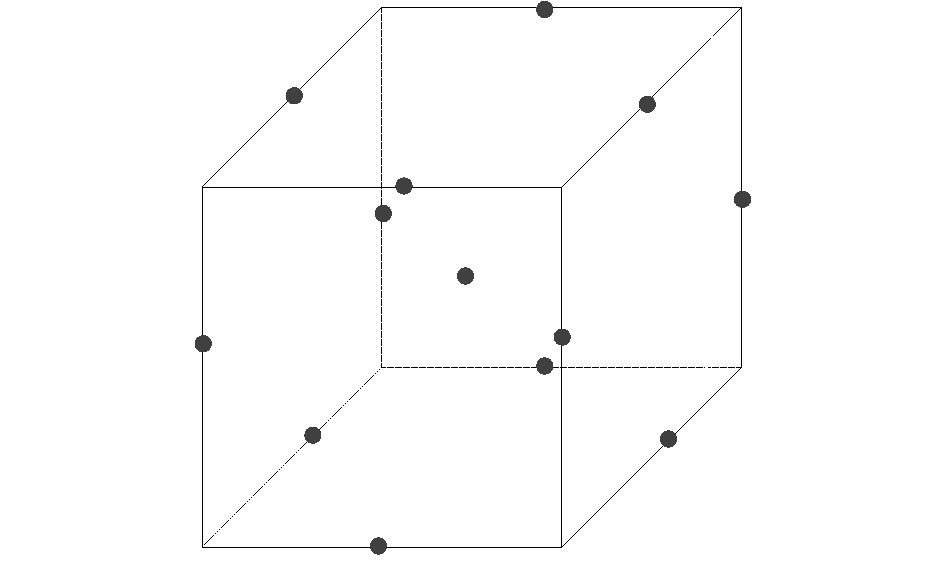
\includegraphics[scale=0.65]{Figuras/cubo.pdf} 
    \caption{Planejamento de Box Behnken.}  
    \legend{Fonte: Adaptado de \citeonline{FERREIRA2007179}}
    \label{fig:cubo}  
\end{figure}

Através da configuração da matriz de Box Behnken é possível obter a Superfície de reposta com os termos lineares, termos com interação e termos quadráticos. Os pontos fatoriais da matriz presentes nas arestas são responsáveis por fornecerem as informações para modelagem de primeira ordem, obtendo os termos lineares e de interações do sistema. Por outro lado, os pontos centrais permitem estimativas dos termos
termos quadráticos da superfície de resposta. O número total de simulações realizadas para a matriz de Box Behnken é \textit{N = 2 * k * (k $-$ 1) + Co}, em que \textit{k} é o número de atributos e \textit{Co} é o número de pontos centrais \cite{box}. 

Através das combinações de atributos geradas a partir da matriz de Box Behnken são efetuadas simulações fluidodinâmicas, o que possibilita a obtenção das respostas da função-objetivo. Após a obtenção da matriz completa com as respectivas respostas, é efetuada a obtenção dos coeficientes de regressão e avaliação estatística dos termos do modelo.

A análise dos termos para os planejamentos estatísticos (Box Behnken e Plackett Burmann) é realizada através de validação estatística, por meio da tabela ANOVA (Análise de variância). Os termos lineares, de interação e quadráticos são considerados significativos para a função-objetivo caso apresentem significância estatística, através do teste \textit{p} e teste F de Fischer presentes na Análise de variância. O teste \textit{p} é um método estatístico que testa a validade da hipótese nula acerca de uma população. Quanto menor o valor-\textit{p}, maior a evidência que a hipótese nula deve ser rejeitada e que a hipótese alternativa pode ser mais confiável. Comumente os níveis alfa são definidos em 5\% ou menos, que se traduzem em intervalos de confiança de 95\% ou mais. Em outras palavras, um valor-\textit{p} inferior a um nível alfa de 5\% significa que existe mais de 95\% de chance de que os resultados não sejam aleatórios e sejam, de fato, significativos estatisticamente. 

A fim de verificar se o modelo se ajusta bem aos dados, são examinadas diversas medidas de adequação. Uma das premissas de um modelo de regressão é a de que os resíduos do modelo devem seguir uma distribuição normal \cite{montgomery}. Para tanto, o teste de normalidade de Kolmogorov-Smirnov é utilizado para avaliar a adequação dos resíduos dos modelos a uma distribuição normal. A hipótese nula deste teste é que os resíduos seguem uma distribuição normal, enquanto a hipótese alternativa é que não seguem. Deste modo, o valor-p resultante é comparado com um nível de significância de 0,05 para determinar se a hipótese nula pode ser rejeitada ou não. Se o valor-p for maior que 0,05, os resíduos são considerados adequados para uma distribuição normal. Caso contrário, os resíduos não são considerados adequados para uma distribuição normal.

Outra análise necessária para o modelo de regressão é a de homocedasticidade dos resíduos do modelo. A homocedasticidade é uma característica estatística que se refere à igualdade da variância dos erros em um modelo estatístico em toda a amplitude dos valores preditores, ou seja, das variáveis independentes. Em outras palavras, a homocedasticidade indica que a dispersão dos erros em torno da linha de regressão é constante em todos os níveis da variável independente. É uma suposição importante em muitos modelos estatísticos, incluindo análises de regressão. Pois a falta de homocedasticidade pode levar a estimativas imprecisas e tendenciosas. Uma maneira comum de avaliar a homocedasticidade é através de gráficos de dispersão dos resíduos em relação às variáveis independentes, onde uma distribuição uniforme sugere homocedasticidade e uma tendência clara dos resíduos indica heterocedasticidade \cite{myers}.

No teste F de Fischer, os valores calculados F para os termos do modelo são comparados com os valores F tabelados de uma distribuição de referência, de acordo com um nível alfa, comumente definido em 5\% e um intervalo de confiança de 95\%. Portanto, um termo é considerado significativo para a variável de resposta do modelo se o F calculado do termo for maior que o F tabelado em um determinado intervalo de confiança e para um determinado Grau de liberdade.


% \subsection{Aprendizado de máquina \textit{(Machine Learning)}} 

% Aprendizado de máquina (ML), são recursos computacionais para desenvolver reconhecimento de padrões, de forma automatizada, a partir de dados de entrada. Os modelos computacionais são desenvolvidos com o objetivo de adquirir informação, realizar inferências e tomar decisões a partir de conjuntos de dados através de métodos estatísticos. Uma característica notável da modelagem de aprendizado de máquina é lidar com problemas multivariados, ou seja, que envolvem diversas variáveis em diferentes escalas \cite{shalev}. Os métodos de aprendizado de máquina podem ser categorizados em: aprendizado supervisionado, aprendizado não supervisionado e aprendizado por reforço.  


% \subsubsection{Aprendizado de máquina supervisionado}  

% Os métodos de aprendizado supervisionado, que é foco desse trabalho, incluem algoritmos que coletam amostras de dados (dados de treino) e suas saídas associadas (\textit{output} ou resposta) para gerar o treinamento do modelo computacional. Esses métodos são chamados de supervisionados, pois o modelo aprende a partir de amostras de dados onde as respostas de saída (\textit{output}) são conhecidas antes de iniciar o processo de modelagem. O objetivo principal é desenvolver um mapeamento ou associação entre amostras de dados de entrada “x” e suas saídas correspondentes “y” com base em várias instâncias de dados de treino. Os modelos podem posteriormente ser usados para a predição do valor do atributo alvo para qualquer nova amostra de dados de entrada \cite{sbsi}. Existem diversos algoritmos de aprendizado supervisionado, tais como: \textit{ Random Forest (RF), Support Vector Machines (SVM), K-Nearest Neighbor (KNN), Decision Tree (DT), Catboost (CB)}, entre outros.  

% Os métodos de aprendizagem supervisionada possuem duas classes principais chamadas de Classificação e Regressão. A aprendizagem supervisionada por classificação possui objetivo principal de prever respostas de natureza categórica para os dados de entrada, com base no que o modelo aprendeu na fase de treinamento. Ou seja, cada resposta de saída do modelo pertence a uma classe ou categoria discreta específica. O método de aprendizagem supervisionada por regressão, é caracterizado por modelos de ML treinados em amostras de dados de entrada em que as respostas são valores numéricos e contínuos. Os modelos de regressão fazem uso de atributos ou recursos de dados de entrada (também chamados de variáveis explicativas ou independentes) e suas valores de saída numéricos e contínuos\cite{james}.  

% \subsubsection{Amostragem de dados por hipercubo latino}  

% Algumas etapas deste trabalho requerem o treinamento de algoritmos de Machine Learning, para tanto é necessário a geração de amostras de dados, ou seja, dados de treino que possuam as respostas do processo que se objetiva modelar. O Hipercubo Latino é um método de amostragem de números aleatórios que visa distribuir a obtenção de amostras de forma uniforme sobre o espaço amostral, ou seja, a seleção de valores aleatórios é realizada de forma dependente \cite{mackay}. A distribuição do atributo é dividia em n regiões diferentes, com igual probabilidade de ocorrência, e seleciona aleatoriamente um valor de cada região para obter uma amostra de tamanho n (Figura \ref{fig:hipercubolatino}).  


% \begin{figure}[H] 
%     \centering  
%     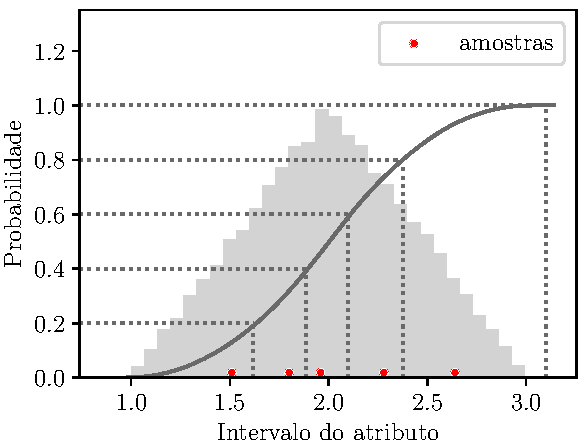
\includegraphics{Figuras/hipercubolatino.pdf}  
%     \caption{Amostragem por Hipercubo Latino.}  
%     \legend{Fonte: Adaptado de \citeonline{mackay}.}
%     \label{fig:hipercubolatino}  
% \end{figure}

% No exemplo mostrado na Figura \ref{fig:hipercubolatino}, para obtenção de 5 amostras de um determinado atributo incerto, a distribuição foi dividida em 5 estratos de igual probabilidade e em cada estrato obtido um valor aleatório. Portanto, conforme o número de amostras aumente, a faixa de valores obtidos por amostragem fica mais próxima da distribuição original.

% \subsubsection{Métodos \textit{ensemble}}


%   Os métodos de aprendizado de máquina \textit{ensemble} são técnicas que criam vários modelos e depois os combinam de alguma forma para produzir melhores resultados. Os métodos de conjunto geralmente produzem soluções mais precisas do que um único modelo. Estes métodos surgiram pois em muitos casos modelos que possuem bons resultados em dados de treinamento, nem sempre oferecem bom desempenho para previsão de novos dados (desconhecidos). Deste modo, a combinação de modelos base podem aumentar a probabilidade de predições satisfatórias em novos dados que não se assemelham aos de treinamento \cite{polikar}. Existem diversos métodos ensemble para combinação de algoritmos, como por exemplo: \textit{bagging, boosting e voting.}

% O método \textit{bagging} divide o conjunto de dados em subconjuntos para treinamento de diferentes algoritmos. Deste modo, para uma modelagem de classificação, a predição da maioria dos modelos é definida como resultado do modelo \textit{ensemble}. No caso de modelagem de regressão, é obtida a média do resultado de todos modelos como predição final para o modelo ensemble. O \textit{Random Forest} é um método de \textit{bagging} com algumas especificidades, que utiliza Árvores de decisão para predição (Figura \ref{fig:randomforest}). De acordo com \cite{breiman}, o método de \textit{Random Forest} utiliza Árvores de decisão distintas para cada subamostragem do conjunto de dados, com objetivo de combinar seus resultados para melhor estimativa de predição final.

% \begin{figure}[H] 
%     \centering  
%     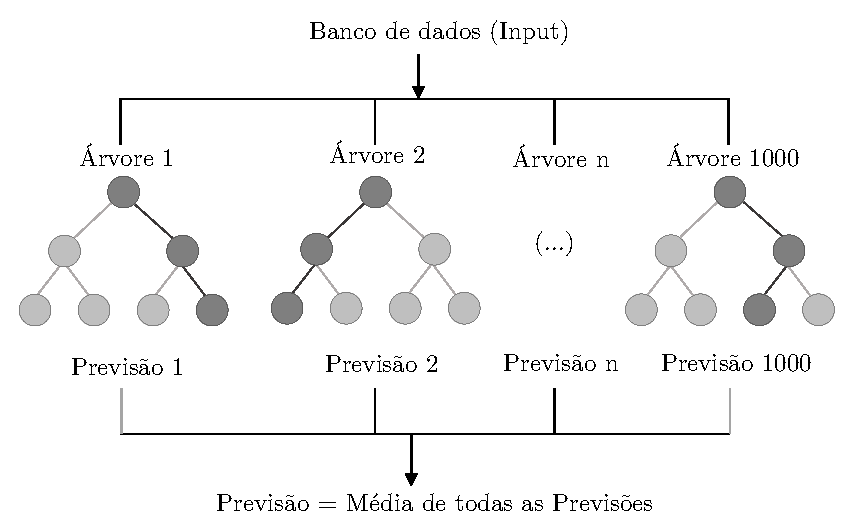
\includegraphics{Figuras/random forest.pdf}  
%     \caption{Método Bagging de regressão por Random Forest.}  
%     \legend{Fonte: Adaptado de \citeonline{breiman}.}
%     \label{fig:randomforest}  
% \end{figure}


% O método de \textit{boosting} treina os modelos de aprendizado de máquina em diferentes dados de treinamento, assim como no método de \textit{bagging}.  Porém, os modelos utilizados no \textit{boosting} aprendem sequencialmente, ou seja, cada algoritmo busca minimizar os erros do modelo anterior. Deste modo, modelos fracos contribuem para criação de modelos preditores mais eficazes, conforme demonstrado na Figura \ref{fig:boosting}. Diferentemente dos modelos \textit{bagging}, a predição de cada algoritmo é ponderada com base em seu desempenho, deste modo os modelos não possuem o mesmo peso na predição final. Existem diversos algoritmos que se baseiam no método de \textit{boosting}, como Catboost, Adaboost, LightGBM, XGBoost entre outros \cite{chen2016}.

% \begin{figure}[H] 
%     \centering
%     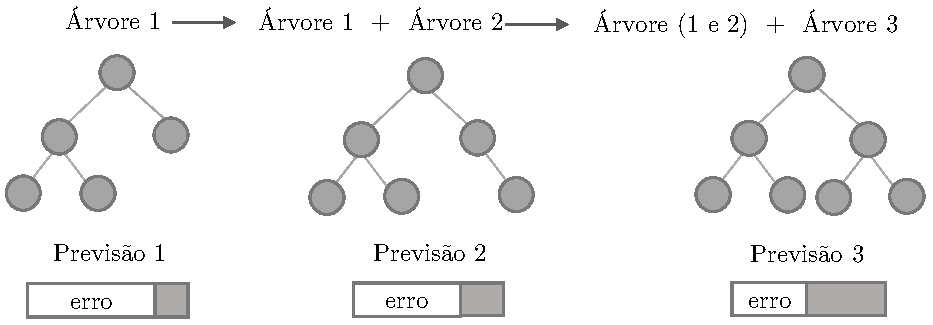
\includegraphics{Figuras/boosting.pdf}
%     \caption{Método Boosting de regressão pelo algoritmo Catboost.}
%     \label{fig:boosting}
%     \legend{Fonte: Adaptado de \citeonline{chen2016}.}
% \end{figure}

% Os métodos de \textit{voting}, podem combinar modelos de diferentes algoritmos para realizar predições. Ao contrário dos modelos de \textit{boosting} e \textit{bagging} que necessitam de modelos de um mesmo tipo. Deste modo, algoritmos diferentes como Support Vector Machines e Árvores de decisão podem ser combinados para realizar uma predição, por exemplo. O resultado final é baseado na maioria dos votos dos algoritmos utilizados \cite{yaman2018}.


% \subsubsection{Aprendizado de máquina automatizado (AutoML)}  

% O crescente uso do aprendizado de máquina em aplicações trouxe consigo a necessidade de automatizar cada vez mais as tarefas de desenvolvimento, visando simplificar as etapas de pré-processamento de dados e criação de modelos preditivos e tornar a prática de aprendizado de máquina mais eficiente. O aprendizado de máquina automatizado (AutoML) é o processo de automatizar as tarefas de aplicação do aprendizado de máquina que seleciona automaticamente os algoritmos para a criação de modelos e quais hiperparâmetros devem ser ajustados para melhorar o desempenho da máquina. O AutoML inclui potencialmente todos os estágios, desde o início com um conjunto de dados brutos até a criação de um modelo de aprendizado de máquina pronto para implantação \cite{balaji2018}. Automatizar o processo de aplicação de aprendizado de máquina oferece as vantagens de produzir soluções mais simples, criação mais rápida dessas soluções e modelos que geralmente superam os modelos projetados de forma padrão. Existem algumas bibliotecas na linguagem Python de código aberto para o \textit{pipeline} de desenvolvimento que oferecem estruturas de autoML para preparações de dados em modelos adaptáveis. Esses \textit{frameworks} automatizam, por exemplo, imputações de valores ausentes, transformações de dados, ajustes de hiperparâmetros e avaliação dos resultados com métricas específicas \cite{elshawi2019}. 

% O PyCaret é um \textit{framework} de aprendizado de máquina e gerenciamento de modelos de código aberto em linguagem de programação Python que automatiza fluxos de trabalho, o que reduz o tempo dedicado na programação de códigos. O PyCaret é essencialmente um compilado em Python de várias bibliotecas e estruturas de aprendizado de máquina que incluem os algoritmos tradicionais e \textit{ensemble}, como scikit-learn, XGBoost, LightGBM, CatBoost, spaCy, Optuna, Hyperopt, Ray entre outras. Comparado com outras bibliotecas de aprendizado de máquina de código aberto, o PyCaret é uma alternativa que pode ser usada para substituir centenas de linhas de programação por apenas alguns comandos. Isso torna os projetos exponencialmente rápidos e eficientes \cite{iqbal2021}.   


\subsubsection{Métricas de Desempenho dos modelos de regressão}  


As métricas de desempenho são cálculos realizados com objetivo de analisar a capacidade preditiva de modelos de regressão. Para modelagens em que os atributos de resposta apresentam variável numérica e contínua, o RMSE é uma métrica frequentemente utilizada. Seu cálculo consiste na raiz quadrada da média dos erros quadrados, entre os valores reais e os previstos pelo modelo, de acordo com a equação \ref{eqn:rmse}.  Quanto maior o valor de RMSE, pior o modelo preditivo.  

  
\begin{equation} 
RMSE = \left ( \frac{1}{n} \sum_{i=1}^{n} ({yi}-\hat{yi})^2 \ \right )^{1/2}  
    \label{eqn:rmse} 
\end{equation} 

Onde:

yi= valor verdadeiro;

$\hat{yi} = \textrm{valor previsto};$

n= tamanho da amostra.

\vspace{1cm}

O cálculo da métrica RMSE eleva a média dos erros do modelo ao quadrado. Assim, diferenças que sejam menores apresentam menor impacto no cálculo, enquanto diferenças maiores recebem mais peso. Outra métrica de regressão amplamente utilizada é o MAE, demonstrado na equação \ref{eqn:mae}. A equação atribui o mesmo peso a todas as diferenças, pois não são elevadas ao quadrado. Deste modo, diferenças grandes e pequenas apresentam o mesmo peso no cálculo da métrica.  


\begin{equation} 
    MAE = \frac{1}{n} \ \sum_{i=1}^{n} | yi - \hat{yi}|  
    \label{eqn:mae} 
\end{equation} 

Onde:

yi= valor verdadeiro;

$\hat{yi} = \textrm{valor previsto};$

n= tamanho da amostra.
\vspace{1cm}

% O MAPE é uma métrica que calcula a média percentual do desvio absoluto entre as predições e os dados observados (equação \ref{eqn:mape}). Essa medida fornece um valor porcentual da média que do quanto o modelo erra nas previsões. Por exemplo, um modelo de regressão com MAPE de 20\% significa que, em média, as previsões erram em 20\% do valor verdadeiro. Ou seja, quanto menor o valor, mais preciso é o modelo de regressão.  

  

%   \begin{equation} 
%       MAPE = \frac{1}{n} \ \sum_{i=1}^{n} | \frac{yi - \hat{yi}}{yi}|  
%       \label{eqn:mape} 
%   \end{equation} 
  

% Onde:

% yi= valor verdadeiro;

% $\hat{yi} = \textrm{valor previsto};$

% n= tamanho da amostra.


% \vspace{1cm}
  Outra métrica comum é o coeficiente de determinação R². Que consiste em uma medida estatística que representa a proporção da variância de uma variável dependente que é explicada por uma variável ou variáveis independentes em um modelo de regressão (equação \ref{eqn:r2}). O R² explica até que ponto a variância de uma variável explica a variância da uma segunda variável. 
  
  \begin{equation}
      R^{2}= 1 - \frac{\sum yi-\hat{yi}}{\sum yi - \overline{y}}
      \label{eqn:r2} 
  \end{equation}


Onde:

yi= valor verdadeiro;

$\hat{yi} = \textrm{valor previsto};$

\={y} = \textrm{média}.$


